

\section{Discussion}

\subsection{Explaining Traversal Variations in Chemistry}
\label{subsection:trav}

Increasing DSi concentration with decreasing elevation suggests the springs are sampling increasingly longer flow paths. This is because longer flow paths allow for more water-rock interaction, which scavenges more DSi from the silicate rocks. While most traverses show such a trend, this does not happen in Traverse 1. One possible reason is that the lowermost springs are likely to be close to the Melamchi river; this is more dilute than the most concentrated springs in the traverse. Mixing with the river waters is possible but unlikely because of the difference in elevation. It is unlikely that the decrease is caused by a dilution effect at the start of the monsoon such as that shown in Figure \ref{fig:time_series_changes}. This is because these DSi trends are consistent across multiple seasons within error. Clearly, however, samples collected in September will be relatively more dilute than those collected in April.

\bsk

A decrease in DSi at lower elevations here could also suggest precipitation of secondary minerals, which is apparent from the Na$^+$/DSi ratio. Linear trends in plot (b) for Traverses 1, 3, and 5 show an increase in Na$^+$/DSi as elevation decreases. Elevated Na$^+$/DSi is interpreted as a sign of a closer approach to equilibrium. Si is involved in kaolinite precipitation whilst Na$^+$ is not, as evidenced in equation \ref{eq:9}, so an increase in their ratio suggests more kaolinite is precipitating \parencite{gaillardetGlobalSilicateWeathering1999}. Kaolinite precipitation is considered to be the backwards reaction, so its increase points to an approach towards equilibrium.

\bsk

Plots of Na$^+$/DSi against elevation can also be used to infer how consistently a given flow path is sampled. Because Na$^+$/DSi is primarily controlled by the balance of dissolution and reprecipitation, and by extension the average age of water in the flow path, consistency of this value over time points to the same flow path length being sampled for a given rate of reaction. Under the steady state assumption assumption $\partial C/\partial t = 0$ used in the residence time models, the Na/DSi ratio should be constant over time at a given elevation if the same flow path is sampled \parencite{lichtner}. For both Traverse 3 and 5, the Na$^+$/DSi ratio against elevation does not change between different seasons. However, there is a better correlation in Traverse 3 which suggests that the flow paths are more consistently sampled there.



\subsection{Residence Time Agreement with Gas Ages}

As shown in Figures 5-9 (c), predicted residence times in the catchment are consistent between the Maher and Fontorbe Models. Residence times increase as elevation decreases, agreeing with the notion that springs sampled at these lower elevations reflect longer flowpaths. Residence times also generally increase with decreasing traversal number, such that Traverse 5 has the lowest and Traverse 1 has the highest. Consistently increasing residence times like this could suggest catchment-wide plumbing, whereby traversal flow paths are interconnected.

\bsk

Residence times in Traverse 3 can be directly compared to the gas ages obtained by \textcite{atwoodCriticalZoneResponse2023}, because both studies are sampling the same springs. The \textcite{atwoodCriticalZoneResponse2023} ages in Traverse 3 range from 5-35 years. The findings from this study and both models predict residence times of a similar order of magnitude. This study does predict older times at the lowest elevation, but these are mostly within the range of propagated uncertainty. Using spring chemistry is therefore a viable method to determine residence times in natural catchments, with the premise that the model assumptions are valid. In addition, this study lends credibility to the use of gas ages to determine residence times, which is an approach that is often criticised for using biased age distributions \parencite{mccallumLimitationsUseEnvironmental2015}. Findings of residence times on the order of 10-100 years for the whole catchment also inform precipitation-discharge relationships. If this study's findings are correct, then the delay in river discharge found by \textcite{andermannImpactTransientGroundwater2012} is likely only recording surface or near-surface flow. The shorter flow paths here could plausibly be associated to residence times of a few months.

\bsk

The fact that both the kinetic-dependent rate Maher model and the kinetics-independent rate Fontorbe model agree with \textcite{atwoodCriticalZoneResponse2023} suggests that the groundwater in Traverse 3 does not get near equilibrium. Reaction rate is kept constant in the Fontorbe model assuming a far from equilibrium state. In the Maher model, reaction rate depends on the equilibrium concentration. As this concentration is reached in the Maher model, the reaction rate will decrease. When the system is far from equilibrium, both models will predict similar times. In order to do test this further, the free energy of the system can be calculated.


\subsection{Free Energy Calculations Concur on Far From Equilibrium State}

\textcite{maherRoleFluidResidence2011} uses their model to conclude that all flow paths reach equilibrium. The free energy of reaction, calculated using the activity of the ions in solution, can be used in natural systems to determine the extent to which equilibrium is reached (\cite{kampmanFeldsparDissolutionKinetics2009}; \cite{wojtowiczThermodynamicBasisSaturation}). Free energies lower than -10 kJ/mol are considered close to equilibrium, whilst those more negative than -40 kJ/mol are categorised as far from equilibrium \parencite{kampmanFeldsparDissolutionKinetics2009}. This method can therefore test the validity of the Maher model in Melamchi. Free energy is defined as:

\begin{equation}
    \Delta G = \Delta G^0 + RT \ln Q
    \label{eq:deltag}
\end{equation}\\

Where in equation \ref{eq:deltag}, $\Delta G$ represents the Gibbs free energy change of reaction, $\Delta G^0$ is the standard Gibbs free energy change, $R$ is the universal gas constant, $T$ denotes the absolute temperature in kelvins, and $Q$ is the reaction quotient. As discussed in the Methods \ref{subsection:weathering}, the weathering reaction characterising this catchment is the dissolution of plagioclase (An-20) and the precipitation of kaolinite, given by equation \ref{eq:9}. The exact composition of plagioclase is important for these calculations. The free energy of reaction is lowered by the presence of a solid solution between albite and anorthite \parencite{dubacqThermodynamicsOrderingMixing2022}. The parameters for the standard free energy of reaction are calculated using the pygcc python package \parencite{awolayoPyGeochemCalcPython2022}. The package gives the standard properties of solid-solution species and reactions, such that $\Delta G^0$ can be calculated:

\begin{equation}
    \Delta G^0 = \Delta G^0_{products} - \Delta G^0_{reactants} = -RT \ln K
\end{equation}

K is calculated using the database obtained from pygcc using The Geochemist's Workbench® Rxn program \parencite{bethkeGEOCHEMICALBIOGEOCHEMICALREACTION}. Q is calculated as the ion activity product of the reaction, assuming the activities of the solid phases plagioclase and kaolinite are 1, the activity of water is 1, and the activity of the ions in solution are equal to their concentration.

\begin{equation}
    Q = \frac{a_{\mathrm{Kaol}}^{0.6}\,a_{\mathrm{Na}^{+}}^{0.8}\,a_{\mathrm{Ca}^{2+}}^{0.2}\,a_{\mathrm{SiO_{2}(aq)}}^{1.6}}
           {a_{\mathrm{An_{20}}}\,a_{\mathrm{H}^{+}}^{1.2}}
\end{equation}


\begin{figure}[H]
    \centering
    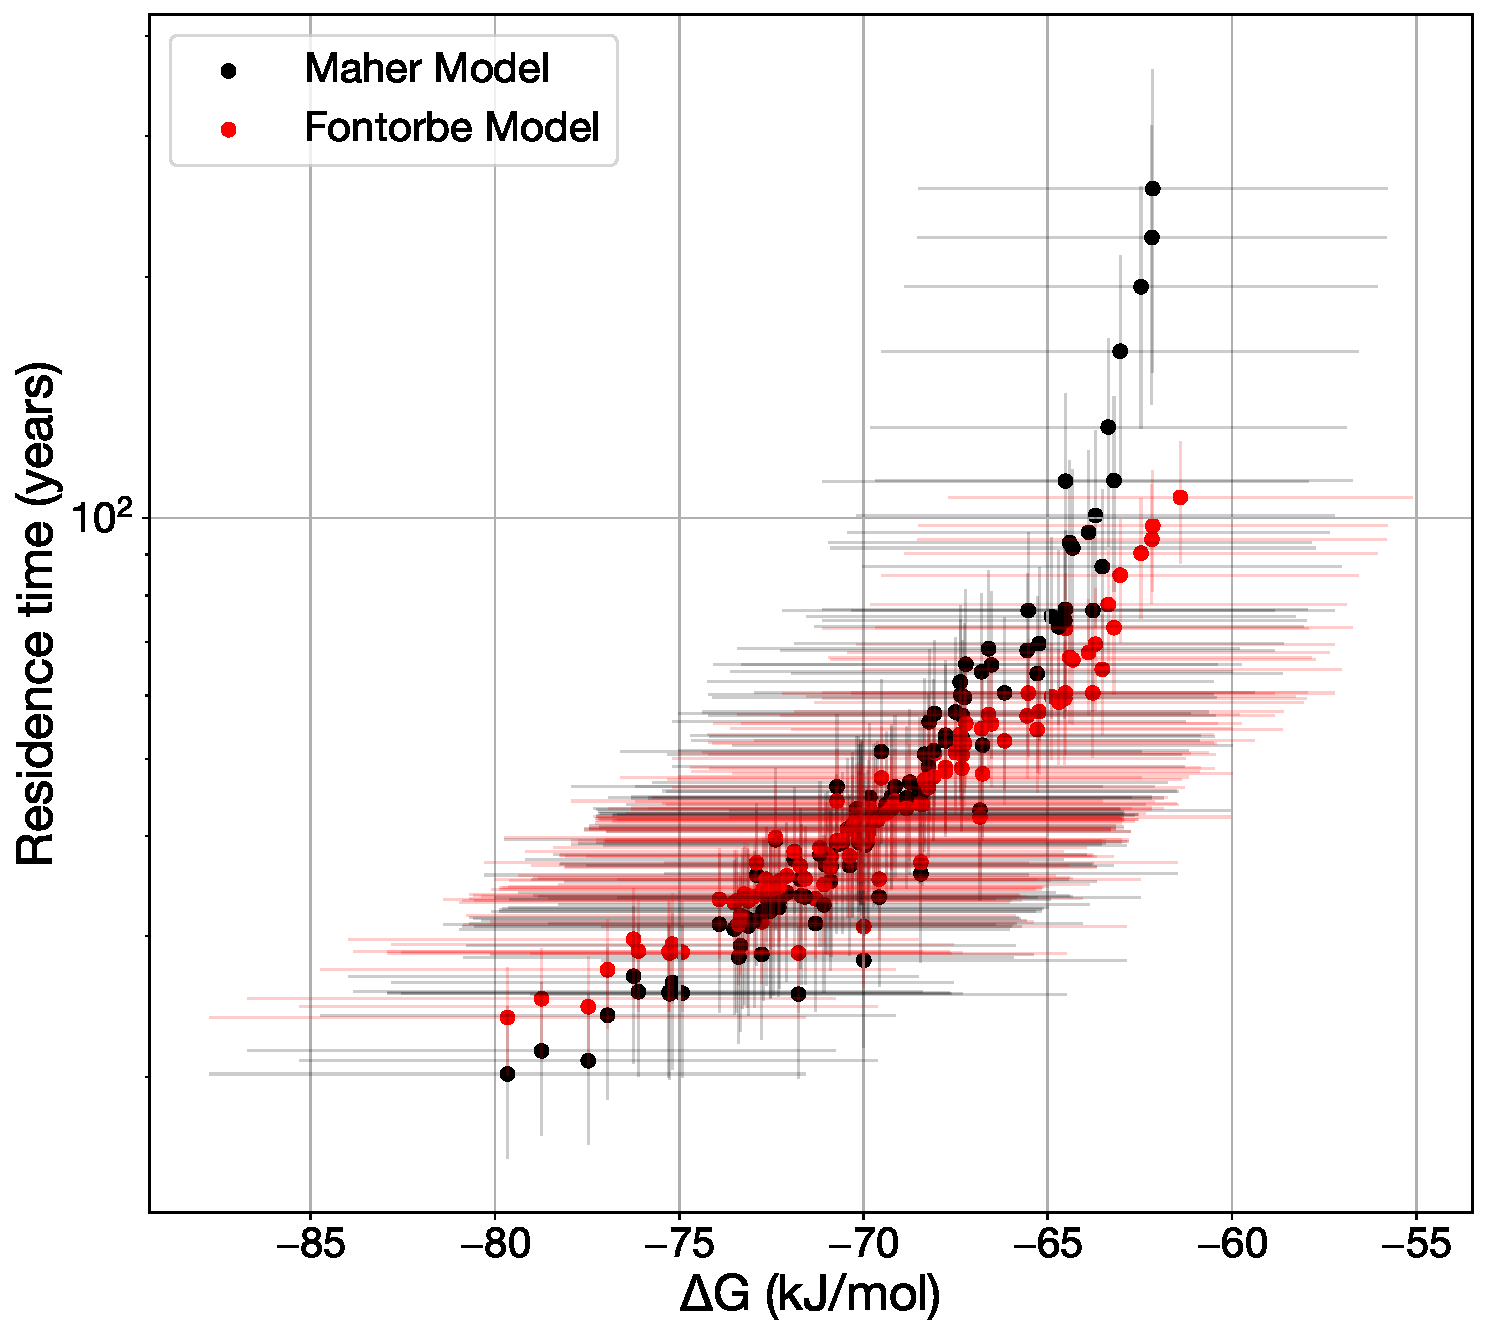
\includegraphics[width=0.8\textwidth]{DGMF.pdf}
    \caption{Estimated residence time against calculated free energy of reaction. Error bars represent Monte Carlo propagated uncertainty. Red points plot the Fontorbe model, while black points plot the Maher model.}
    \label{fig:deltag}
\end{figure}

\FloatBarrier

Figure \ref{fig:deltag} shows that all springs in the catchment have a free energy that is more negative than -60 kJ/mol. These samples are therefore classified as far from equilibrium. Note that being far from equilibrium is not inconsistent with evidence for secondary precipitation as shown in Figures \ref{fig:modal}, \ref{fig:trav1}-\ref{fig:trav5}; simply, being closer to equilibrium would suggest more precipitation. Figure \ref{fig:deltag} does show that free energy gets closer to zero as residence time increases. This is consistent with the notion that groundwaters approach equilibrium the more they stay in the subsurface and react. However, the extent of reaction is not great enough to be considered close to equilibrium. This suggests that, for Melamchi, using the Maher model to estimate residence times is not appropriate.


% \caption{Summary of free energy results from each traverse. Standard deviation corresponds to Monte Carlo propagated uncertainty.} \\
% \label{tab:delta_G}\\

% Begin two-column layout


\begin{landscape}
    
    \begin{table}
        \caption{Summary of free energy results from each traverse. Standard deviation corresponds to Monte Carlo propagated uncertainty.}
        \label{tab:delta_G}
        \scriptsize  % Apply scriptsize to the entire table
        \setlength\tabcolsep{2mm}
        \begin{tabular}{M{.30\textwidth} @{\hspace{4cm}} M{.30\textwidth} @{\hspace{4cm}} M{.30\textwidth}}
            % First column - Transactions Table
            \begin{tabular}{l l l l l}
    \textbf{Sample ID}  &  \textbf{Season}  &  \textbf{Traverse}  &  \textbf{Elevation}  &  \textbf{$\Delta$G $\pm$ 1$\sigma$} \\
    \hline
    &   &   &  \textbf{m}  &  \textbf{kJ/mol} \\
    \hline
    NEP24-001 & Sep 24 & Traverse 1 & 928 & -69.7 ±  7.1 \\
    NEP22-87 & Nov 22 & Traverse 1 & 1270 & -68.5 ±  7.0 \\
    MKS 1B & Nov 18 & Traverse 1 & 1432 & -68.2 ±  7.0 \\
    NEP22-86 & Nov 22 & Traverse 1 & 1124 & -66.5 ±  6.8 \\
    NEP24-003 & Sep 24 & Traverse 1 & 876 & -65.6 ±  6.7 \\
    NEP22-2 & Nov 22 & Traverse 1 & 890 & -65.3 ±  6.7 \\
    MKS-1 & Nov 18 & Traverse 1 & 1433 & -64.6 ±  6.6 \\
    NEP24-002 & Sep 24 & Traverse 1 & 868 & -64.6 ±  6.6 \\
    NEP22-85 & Nov 22 & Traverse 1 & 1195 & -64.5 ±  6.6 \\
    MKS-3 & Nov 18 & Traverse 1 & 1152 & -64.4 ±  6.6 \\
    NEP22-1 & Nov 22 & Traverse 1 & 871 & -63.8 ±  6.5 \\
    MKS-24 & Nov 18 & Traverse 1 & 850 & -63.6 ±  6.5 \\
    NEP22-80 & Nov 22 & Traverse 1 & 1046 & -63.4 ±  6.5 \\
    NEP22-81 & Nov 22 & Traverse 1 & 1207 & -63.1 ±  6.4 \\
    NEP22-82 & Nov 22 & Traverse 1 & 1212 & -62.5 ±  6.4 \\
    NEP22-83 & Nov 22 & Traverse 1 & 1244 & -62.3 ±  6.4 \\
    MKS-2 & Nov 18 & Traverse 1 & 1083 & -62.2 ±  6.4 \\
    \specialrule{0.2pt}{1pt}{1pt}
    NEP24-061 & Sep 24 & Traverse 2 & 1527 & -76.4 ±  7.8 \\
    NEP22-61 & Nov 22 & Traverse 2 & 1524 & -76.3 ±  7.7 \\
    NEP24-062 & Sep 24 & Traverse 2 & 1452 & -72.5 ±  7.4 \\
    NEP22-62 & Nov 22 & Traverse 2 & 1504 & -71.8 ±  7.3 \\
    NEP22-79 & Nov 22 & Traverse 2 & 1277 & -71.8 ±  7.3 \\
    NEP22-63 & Nov 22 & Traverse 2 & 1447 & -71.4 ±  7.3 \\
    NEP22-66 & Nov 22 & Traverse 2 & 1359 & -71.0 ±  7.2 \\
    \hline
    \end{tabular}
    &
    % Second column
    \begin{tabular}{l l l l l}
        \setlength\tabcolsep{0.1cm}
\textbf{Sample ID}  &  \textbf{Season}  &  \textbf{Traverse}  &  \textbf{Elevation}  &  \textbf{$\Delta$G $\pm$ 1$\sigma$} \\
\hline
&   &   &  \textbf{m}  &  \textbf{kJ/mol} \\
\hline
    NEP22-65 & Nov 22 & Traverse 2 & 1429 & -70.8 ±  7.2 \\
    NEP24-065 & Sep 24 & Traverse 2 & 1129 & -70.1 ±  7.1 \\
    NEP24-063 & Sep 24 & Traverse 2 & 1285 & -68.8 ±  7.0 \\
    NEP22-64 & Nov 22 & Traverse 2 & 1442 & -68.3 ±  7.0 \\
    NEP22-78 & Nov 22 & Traverse 2 & 1270 & -67.5 ±  6.9 \\
    NEP22-68 & Nov 22 & Traverse 2 & 1288 & -67.4 ±  6.9 \\
    NEP22-67 & Nov 22 & Traverse 2 & 1125 & -66.9 ±  6.8 \\
    NEP24-068 & Sep 24 & Traverse 2 & 949 & -66.9 ±  6.8 \\
    NEP22-77 & Nov 22 & Traverse 2 & 1273 & -66.7 ±  6.8 \\
    NEP24-067 & Sep 24 & Traverse 2 & 1000 & -66.2 ±  6.8 \\
    NEP22-71 & Nov 22 & Traverse 2 & 996 & -65.3 ±  6.7 \\
    MKS-10 & Nov 18 & Traverse 2 & 930 & -65.0 ±  6.7 \\
    NEP22-70 & Nov 22 & Traverse 2 & 950 & -64.8 ±  6.6 \\
    MKS 10B & Nov 18 & Traverse 2 & 929 & -64.6 ±  6.6 \\
    NEP22-76 & Nov 22 & Traverse 2 & 1074 & -64.0 ±  6.6 \\
    NEP22-75 & Nov 22 & Traverse 2 & 1052 & -63.8 ±  6.5 \\
    NEP22-73 & Nov 22 & Traverse 2 & 979 & -63.2 ±  6.5 \\
    \specialrule{0.2pt}{1pt}{1pt}
    NEP24-014 & Sep 24 & Traverse 3 & 2496 & -79.8 ±  8.1 \\
    NEP22-9 & Nov 22 & Traverse 3 & 2522 & -78.9 ±  8.0 \\
    NEP24-015 & Sep 24 & Traverse 3 & 2101 & -75.1 ±  7.6 \\
    NEP24-016 & Sep 24 & Traverse 3 & 1979 & -75.0 ±  7.7 \\
    NEP24-034 & Sep 24 & Traverse 3 & 2415 & -74.9 ±  7.6 \\
    MKS-6 & Nov 18 & Traverse 3 & 2124 & -74.6 ±  7.6 \\
    NEP22-20 & Nov 22 & Traverse 3 & 2104 & -74.6 ±  7.6 \\
    \hline
        \end{tabular}
        &
        % Second column
        \begin{tabular}{l l l l l}
            \setlength\tabcolsep{0.1cm}
    \textbf{Sample ID}  &  \textbf{Season}  &  \textbf{Traverse}  &  \textbf{Elevation}  &  \textbf{$\Delta$G $\pm$ 1$\sigma$} \\
    \hline
    &   &   &  \textbf{m}  &  \textbf{kJ/mol} \\
    \hline
    NEP22-17 & Nov 22 & Traverse 3 & 2102 & -74.0 ±  7.5 \\
    NEP22-12 & Nov 22 & Traverse 3 & 2386 & -73.6 ±  7.5 \\
    NEP22-16 & Nov 22 & Traverse 3 & 1964 & -73.4 ±  7.5 \\
    NEP22-19 & Nov 22 & Traverse 3 & 2097 & -73.4 ±  7.5 \\
    NEP22-13 & Nov 22 & Traverse 3 & 2098 & -73.2 ±  7.5 \\
    NEP22-10 & Nov 22 & Traverse 3 & 2418 & -73.1 ±  7.4 \\
    NEP22-11 & Nov 22 & Traverse 3 & 2418 & -73.0 ±  7.4 \\
    NEP22-46 & Nov 22 & Traverse 3 & 2555 & -72.8 ±  7.4 \\
    MKS 5B & Nov 18 & Traverse 3 & 2428 & -72.5 ±  7.4 \\
    MKS-5 & Nov 18 & Traverse 3 & 2434 & -72.0 ±  7.3 \\
    NEP24-017 & Sep 24 & Traverse 3 & 1990 & -71.8 ±  7.3 \\
    NEP22-15 & Nov 22 & Traverse 3 & 1973 & -70.2 ±  7.2 \\
    NEP22-18 & Nov 22 & Traverse 3 & 2091 & -70.2 ±  7.2 \\
    NEP24-011 & Sep 24 & Traverse 3 & 1318 & -70.1 ±  7.1 \\
    NEP24-010 & Sep 24 & Traverse 3 & 1314 & -70.0 ±  7.1 \\
    MKS-7 & Nov 18 & Traverse 3 & 1805 & -69.8 ±  7.1 \\
    NEP22-55 & Nov 22 & Traverse 3 & 1772 & -69.8 ±  7.1 \\
    NEP22-54 & Nov 22 & Traverse 3 & 1779 & -69.7 ±  7.1 \\
    NEP22-59 & Nov 22 & Traverse 3 & 1324 & -69.5 ±  7.1 \\
    NEP22-53 & Nov 22 & Traverse 3 & 1777 & -69.4 ±  7.0 \\
    NEP22-42 & Nov 22 & Traverse 3 & 1325 & -69.3 ±  7.1 \\
    NEP22-60 & Nov 22 & Traverse 3 & 1160 & -68.5 ±  7.0 \\
    MKS-9 & Nov 18 & Traverse 3 & 1212 & -68.4 ±  7.0 \\
    MKS 9B & Nov 18 & Traverse 3 & 1214 & -67.8 ±  6.9 \\
    \hline
        \end{tabular}\\ % Correct placement of hline after the main row
    \end{tabular}
\end{table}
\end{landscape}

   \newpage

   \begin{landscape}
    
    \begin{table}
        \scriptsize  % Apply scriptsize to the entire table
        \setlength\tabcolsep{2mm}
        \begin{tabular}{M{.30\textwidth} @{\hspace{4cm}} M{.30\textwidth} @{\hspace{4cm}} M{.30\textwidth}}
            % First column - Transactions Table
            \begin{tabular}{l l l l l}
            \textbf{Sample ID}  &  \textbf{Season}  &  \textbf{Traverse}  &  \textbf{Elevation}  &  \textbf{$\Delta$G $\pm$ 1$\sigma$} \\
            \hline
            &   &   &  \textbf{m}  &  \textbf{kJ/mol} \\
            \hline
    NEP22-45 & Nov 22 & Traverse 3 & 1195 & -67.8 ±  6.9 \\
    NEP24-038 & Sep 24 & Traverse 3 & 1408 & -67.6 ±  6.9 \\
    MKS-8 & Nov 18 & Traverse 3 & 1430 & -67.4 ±  6.9 \\
    NEP22-58 & Nov 22 & Traverse 3 & 1447 & -67.4 ±  6.9 \\
    NEP22-56 & Nov 22 & Traverse 3 & 1433 & -66.9 ±  6.8 \\
    \specialrule{0.2pt}{1pt}{1pt}
    MKS 4B & Nov 18 & Traverse 4 & 2524 & -76.3 ±  7.8 \\
    NEP24-050 & Sep 24 & Traverse 4 & 2452 & -73.6 ±  7.5 \\
    NEP22-48 & Nov 22 & Traverse 4 & 2067 & -71.1 ±  7.2 \\
    NEP24-051 & Sep 24 & Traverse 4 & 2076 & -71.0 ±  7.3 \\
    NEP24-041 & Sep 24 & Traverse 4 & 1614 & -70.8 ±  7.2 \\
    MKS-13 & Nov 18 & Traverse 4 & 2077 & -70.7 ±  7.2 \\
    NEP22-47 & Nov 22 & Traverse 4 & 2450 & -70.5 ±  7.2 \\
    MKS-4 & Nov 18 & Traverse 4 & 2521 & -70.3 ±  7.2 \\
    NEP22-52 & Nov 22 & Traverse 4 & 1529 & -69.6 ±  7.1 \\
    NEP24-052 & Sep 24 & Traverse 4 & 1987 & -69.2 ±  7.1 \\
    MKS-12 & Nov 18 & Traverse 4 & 1479 & -68.5 ±  7.0 \\
    NEP22-49 & Nov 22 & Traverse 4 & 1966 & -68.5 ±  7.0 \\
    NEP22-50 & Nov 22 & Traverse 4 & 1698 & -67.4 ±  6.9 \\
    NEP24-040 & Sep 24 & Traverse 4 & 1693 & -67.3 ±  6.9 \\
    NEP22-57 & Nov 22 & Traverse 4 & 1462 & -65.6 ±  6.7 \\
    \specialrule{0.2pt}{1pt}{1pt}
    NEP24-027 & Sep 24 & Traverse 5 & 2858 & -77.6 ±  7.9 \\
    MKS-23 & Nov 18 & Traverse 5 & 3379 & -77.0 ±  7.8 \\
    MKS 21B & Nov 18 & Traverse 5 & 3007 & -76.2 ±  7.7 \\
    NEP22-26 & Nov 22 & Traverse 5 & 2579 & -75.4 ±  7.7 \\
    \hline
    \end{tabular}
    &
    % Second column
    \begin{tabular}{l l l l l}
        \setlength\tabcolsep{0.1cm}

            \textbf{Sample ID}  &  \textbf{Season}  &  \textbf{Traverse}  &  \textbf{Elevation}  &  \textbf{$\Delta$G $\pm$ 1$\sigma$} \\
            \hline
            &   &   &  \textbf{m}  &  \textbf{kJ/mol} \\
            \hline
    NEP22-27 & Nov 22 & Traverse 5 & 3126 & -75.3 ±  7.6 \\
    NEP22-28 & Nov 22 & Traverse 5 & 2954 & -75.3 ±  7.7 \\
    MKS-14 & Nov 18 & Traverse 5 & 2536 & -73.5 ±  7.5 \\
    NEP24-020 & Sep 24 & Traverse 5 & 2556 & -73.5 ±  7.5 \\
    NEP24-028 & Sep 24 & Traverse 5 & 2782 & -73.2 ±  7.4 \\
    NEP22-29 & Nov 22 & Traverse 5 & 2852 & -73.0 ±  7.4 \\
    NEP22-23 & Nov 22 & Traverse 5 & 2517 & -72.9 ±  7.4 \\
    MKS-20 & Nov 18 & Traverse 5 & 1903 & -72.7 ±  7.4 \\
    NEP22-39 & Nov 22 & Traverse 5 & 2523 & -72.6 ±  7.4 \\
    NEP24-025 & Sep 24 & Traverse 5 & 3127 & -72.6 ±  7.4 \\
    NEP22-24 & Nov 22 & Traverse 5 & 2622 & -72.5 ±  7.4 \\
    MKS 22B & Nov 18 & Traverse 5 & 3130 & -72.4 ±  7.4 \\
    NEP22-22 & Nov 22 & Traverse 5 & 2758 & -72.4 ±  7.4 \\
    MKS-22 & Nov 18 & Traverse 5 & 3126 & -72.2 ±  7.4 \\
    NEP22-25 & Nov 22 & Traverse 5 & 2562 & -71.8 ±  7.3 \\
    NEP22-30 & Nov 22 & Traverse 5 & 2757 & -71.7 ±  7.3 \\
    NEP24-022 & Sep 24 & Traverse 5 & 2259 & -71.3 ±  7.3 \\
    NEP22-35 & Nov 22 & Traverse 5 & 2068 & -71.1 ±  7.3 \\
    MKS-17 & Nov 18 & Traverse 5 & 2163 & -71.0 ±  7.2 \\
    MKS 15B & Nov 18 & Traverse 5 & 2000 & -70.4 ±  7.2 \\
    NEP22-32 & Nov 22 & Traverse 5 & 2252 & -70.4 ±  7.2 \\
    NEP24-023 & Sep 24 & Traverse 5 & 2269 & -70.4 ±  7.2 \\
    NEP24-021 & Sep 24 & Traverse 5 & 2243 & -70.3 ±  7.2 \\
    MKS-18 & Nov 18 & Traverse 5 & 2262 & -70.2 ±  7.1 \\
    \hline
    \end{tabular}
    &
    % Second column
    \vtop{
    \begin{tabular}{l l l l l}
        \setlength\tabcolsep{0.1cm}
    \textbf{Sample ID}  &  \textbf{Season}  &  \textbf{Traverse}  &  \textbf{Elevation}  &  \textbf{$\Delta$G $\pm$ 1$\sigma$} \\
    \hline
    &   &   &  \textbf{m}  &  \textbf{kJ/mol} \\
    \hline

    NEP22-33 & Nov 22 & Traverse 5 & 2247 & -70.2 ±  7.1 \\
    MKS 18B & Nov 18 & Traverse 5 & 2265 & -70.1 ±  7.1 \\
    NEP22-31 & Nov 22 & Traverse 5 & 2573 & -70.1 ±  7.1 \\
    NEP22-34 & Nov 22 & Traverse 5 & 2240 & -70.1 ±  7.1 \\
    MKS-16 & Nov 18 & Traverse 5 & 1942 & -70.0 ±  7.1 \\
    MKS-19 & Nov 18 & Traverse 5 & 2164 & -69.9 ±  7.2 \\
    NEP22-37 & Nov 22 & Traverse 5 & 2050 & -69.0 ±  7.0 \\
    NEP22-36 & Nov 22 & Traverse 5 & 1987 & -68.1 ±  6.9 \\
    \hline
        \end{tabular}}\\ % Correct placement of hline after the main row
    \end{tabular}
\end{table}
\end{landscape}

   \newpage


\subsection{Model Sensitivity to Concentration}

Residence times in Traverse 1 are explainably the longest in the catchment. The springs here at are the lowest elevation, so the flow paths are presumably the longest. This is consistent with the highest DSi concentration of the catchment, and evidence for secondary precipitation of kaolinite at the lowest elevations (see Figure \ref{fig:trav1} (b)). In Traverse 1, the Fontorbe model predicts a peak of $\approx$ 100 years, while the Maher model has a much higher residence time of $\approx$ 300 years. The discrepancy is likely due to how the models are formulated.

\begin{table}[h]
    \centering
    \renewcommand{\arraystretch}{2.2} % Adjust row spacing
    \begin{tabular}{cc}
        \toprule
        \textbf{Fontorbe} & \textbf{Maher} \\
        \midrule
        $\displaystyle T_f  = \frac{\left(C_h - C_o\right)\cdot\phi}{\left(1-f\right)\cdot R_n}$ & 
        $\displaystyle T_f = \frac{C_{eq} \cdot \left(C - C_0\right)}{e^2 R_n \left( C_{\text{eq}} - C \right)}$ \\ [10pt]
        \bottomrule
    \end{tabular}
    \caption{Comparison of residence time equations from Fontorbe and Maher.}
    \label{tab:equations}
\end{table}

The difference in the models comes from the underlying assumptions of reaction rate and how it changes towards equilibrium. The Fontorbe assumption that reaction rate remains constant as the reaction progresses is unrealistic, as all weathering reactions are bound to stop at some time. Hence, the Maher model more accurately reflects water in these catchments that is closer to equilibrium. The $\frac{C_{eq}}{(C_{eq} - C)}$ term in the Maher model gets larger as the concentration approaches equilibrium. As a result of this, the Maher model consistently predicts longer residence times than the Fontorbe Model at higher DSi concentrations, while the opposite is true at lower DSi concentrations. For Traverse 1 the $\frac{C_{eq}}{(C_{eq} - C)}$ term grows arbitrarily large, hence the strong discrepancy found in Figure \ref{fig:trav1} (c).

\bsk

For this study's calculations, the equilibrium concentration is taken to be the highest in the catchment, 869 $\mu$M DSi. This concentration corresponds the highest spring concentration found in Traverse 1. Note that in the \textcite{maherHydrologicRegulationChemical2014} model setup, an equilibrium concentration of 375$\mu$M DSi is chosen from the global river data of \textcite{gaillardetGlobalSilicateWeathering1999}. This is sound for a theoretical model but is not appropriate for this catchment. It is unclear, however, whether choosing the highest DSi concentration in the catchment is appropriate. Clearly as this concentration is approached, the Maher model will predict unrealistic residence times, as shown in Figure \ref{fig:deltag}. The free energy of the system suggests the spring system is far away from equilibrium, so choosing a larger $C_{eq}$ would produce better agreement with the Fontorbe model at higher DSi concentrations and allow for the calculated free energy. Additionally, \textcite{maherRoleFluidResidence2011} details several ways in which $C_{eq}$ could change depending on the conditions. For example, increasing pCO$_2$ would increase the concentration of DSi at equilibrium. Another way to potentially estimate the maximum DSi concentration would be to calculate this at equilibrium by simulating further reaction of the most reacted springs with the appropriate minerals. The only assumption here would be that CO$_2$ is conserved. However, if the Maher model assumes that all flow paths reach equilibrium, it is appropriate to use a concentration measured within the catchment; otherwise, applying the model would be of little relevance to the overall discussion on weathering controls.

\begin{figure}[h]
    \centering
    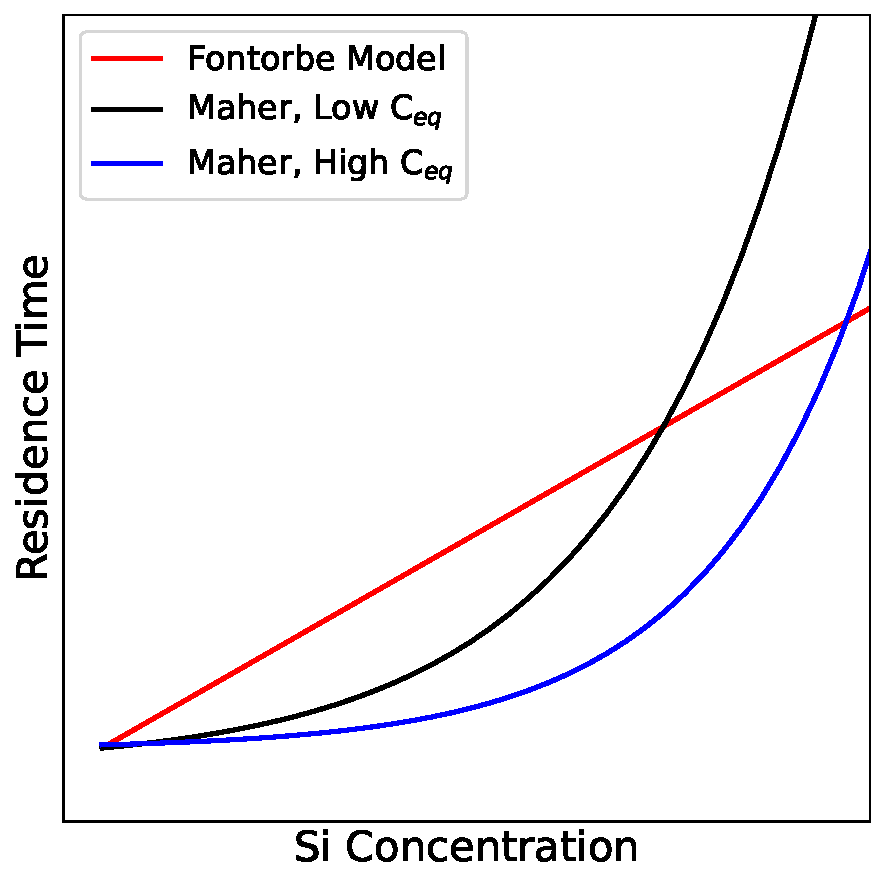
\includegraphics[width=0.6\textwidth]{Linear_vs_Exponential_Comparison.pdf}
    \caption{Illustrative sketch of how dissolved silica concentration changes with flow path length for the two models, and different equilibrium concentration for the Maher model. Plotted lines are taken from the model equations \ref{eq:fontorbe} and \ref{eq:maher}.}
    \label{fig:comparisonceq}
\end{figure}

\FloatBarrier

There is another potential issue related to the dependence of residence time on the concentration of DSi. As is apparent in Figures \ref{fig:trav1}-\ref{fig:trav5} and Table \ref{tab:equations}, the estimated residence time of both models is directly related to the DSi concentration in the spring water. This is by design, however as expressed in subsection \ref{subsection:trav}, low DSi is not necessarily indicative of less reacted groundwater. As a result of this, there is the possibility that the estimated residence times act more as a lower bound. A better approach in a future study could use elemental ratios, for example Na$^+$/DSi that has a known behaviour as the reaction progresses. Elemental ratios like that would also factor out dilution as a potential influencing factor.


\subsection{Is the Rate Constant Used Appropriate?}

Figure \ref{fig:deltag} suggests that the system is far away from equilibrium, but the reaction rate constant used in both models for all calculations is one that is only considered feasible when close to equilibrium \parencite{kampmanFeldsparDissolutionKinetics2009}. In systems far from equilibrium, the reaction rate constant has been suggested to be much larger than those used in the models \parencite{whiteEffectTimeWeathering2003}. Field rate constants lie between 10$^{-13}$ and 10$^{-17}$ mol m$^{-2}$ s$^{-1}$, while laboratory rate constants are between 10$^{-11}$ and 10$^{-13}$ mol m$^{-2}$ s$^{-1}$ \parencite{whiteEffectTimeWeathering2003}. If the rate constant is increased, the residence times predicted by the models will decrease. This is because the rate of reaction is inversely proportional to the residence time, as seen in the equations in Table \ref{tab:equations}. Reaction rate constants that are suggested to be far from equilibrium in \textcite{kampmanFeldsparDissolutionKinetics2009} are laboratory-derived rates, and four orders of magnitude higher than those used in this study. Using these rates for the models predicts residence times in the range of 1-10 days. Under the assumption that the rates displayed in \textcite{kampmanFeldsparDissolutionKinetics2009} are accurate for systems far away from equilibrium, the results no longer agree with \textcite{atwoodCriticalZoneResponse2023}. Under these circumstances, then, the Maher and Fontorbe models are less likely to be appropriate for use in discussing weathering controls. 

\bsk

There are, however, counterarguments to this. Firstly, \textcite{kampmanFeldsparDissolutionKinetics2009} investigate river - not spring - water draining a different lithology, under different pH and pCO$_2$ conditions than Melamchi. Secondly, the reaction rate constants reported at far from equilibrium free energies are calculated in the laboratory, at different conditions to both this study and \textcite{kampmanFeldsparDissolutionKinetics2009}. Field derived reaction rate constants are often found to be lower than those measured in the lab. It is therefore unclear whether the k-$\Delta G$ relationship suggested in \textcite{kampmanFeldsparDissolutionKinetics2009} is applicable to Melamchi, or natural catchments in general. In other words, in the absence of field-derived reaction rate constants in far from equilibrium settings, there is little evidence to suggest that the rate constants used in this study, and the models' calculated residence times are incorrect. This therefore suggests that the Maher and Fontorbe model rate constants are appropriate for use in natural catchments.


\newpage

\section{Conclusions and Future Work}

Elemental concentrations and ratios for different springs in the kinetically-limited Melamchi catchment are reproducible over different field seasons, with dilution in the monsoon season. This suggests that the flow paths coming out of each spring are consistently sampled. Reactive transport models can then be used to estimate residence times in the catchment. Estimated times of order 10-100 years by the Fontorbe and Maher models are consistent with previously obtained gas ages in Melamchi. This study therefore presents a novel approach to predict residence times using the chemistry of spring waters alone. This has implications for predicting weathering controls and resilience to drought in Himalayan catchments. Both models predict similar times at low concentration, suggesting that the system is not close to equilibrium, and free energy calculations agree. The distance of the catchment from equilibrium is inconsistent with the Maher model assumption that all flow paths reach it. The Maher model is likely more appropriate - weathering reactions are ultimately not going to go on indefinitely, so a decreasing reaction rate is a physically realistic assumption. However, the Fontorbe and Maher differ little in Melamchi because the fluids are far from equilibrium at the end of the flow path. Maher's contention that weathering paths always approach equilibrium, and are therefore more sensitive to water flux than temperature, does not hold for Melamchi and by implication other rapidly eroding terrains. Whether this suggests that the greatest control on weathering is temperature is less clear. Calculated free energy is not inconsistent with the Fontorbe model, but this does not mean it is the most appropriate model to use for Melamchi, especially given its reaction rate formulation.


\bsk


There are caveats to these conclusions. Firstly, depending on the equilibrium concentration chosen for the Maher model, the measured concentrations used and predicted times could be consistent with a far from equilibrium system. The choice of this equilibrium concentration is however linked to the natural system it is found in, so choosing the highest measured concentration in the catchment is considered the most appropriate option. Secondly, just using elemental concentrations has the potential to underestimate residence times, as a result of secondary precipitation reactions. Lastly, if the system is far from equilibrium, a corresponding rate constant should be used for the model calculations. These rate constants are orders of magnitude larger than those considered close to equilibrium, and so would lead to predicted residence times on the order of days. Nonetheless it is unclear whether these rate constants are appropriate for natural catchments given they were not estimated in a natural setting.

\bsk

There is significant scope for future work in this area. Elemental ratios are more readily indicative of back-reactions than concentrations alone, and so can be implemented into the models to estimate residence times more accurately. Given model dependence on reaction rate constants, it would be beneficial to quantify a backward reaction rate to add to the forward dissolution rate used in the models. This would allow for secondary precipitation to be accounted for instead of it being a potential source of error. Finally, isotope tracers like $\delta^2$H, $\delta^{18}$O, $\delta^{30}$Si, $^{87}$Sr/$^{86}$Sr, and $\delta^7$Li are often proposed for use together in natural catchments to distinguish old and new water because of their ability to identify different aspects of reaction and mixing \parencite{druhanIsotopeRatioDischarge2023}. 








% Talk about using element ratios, and also isotope tracers eg Jotis, and also different reaction rates for forward and backward



% \bsk

% The consistency with which flow paths are sampled in Traverse 3 is more apparent when plotting Na/Si in one season against the rest (note that Figure \ref{fig:spatial_changes_spring8} the Na/Si values are uncorrected to showcase results collected in more than two seasons). 

% \begin{figure}[h]
%     \centering
%     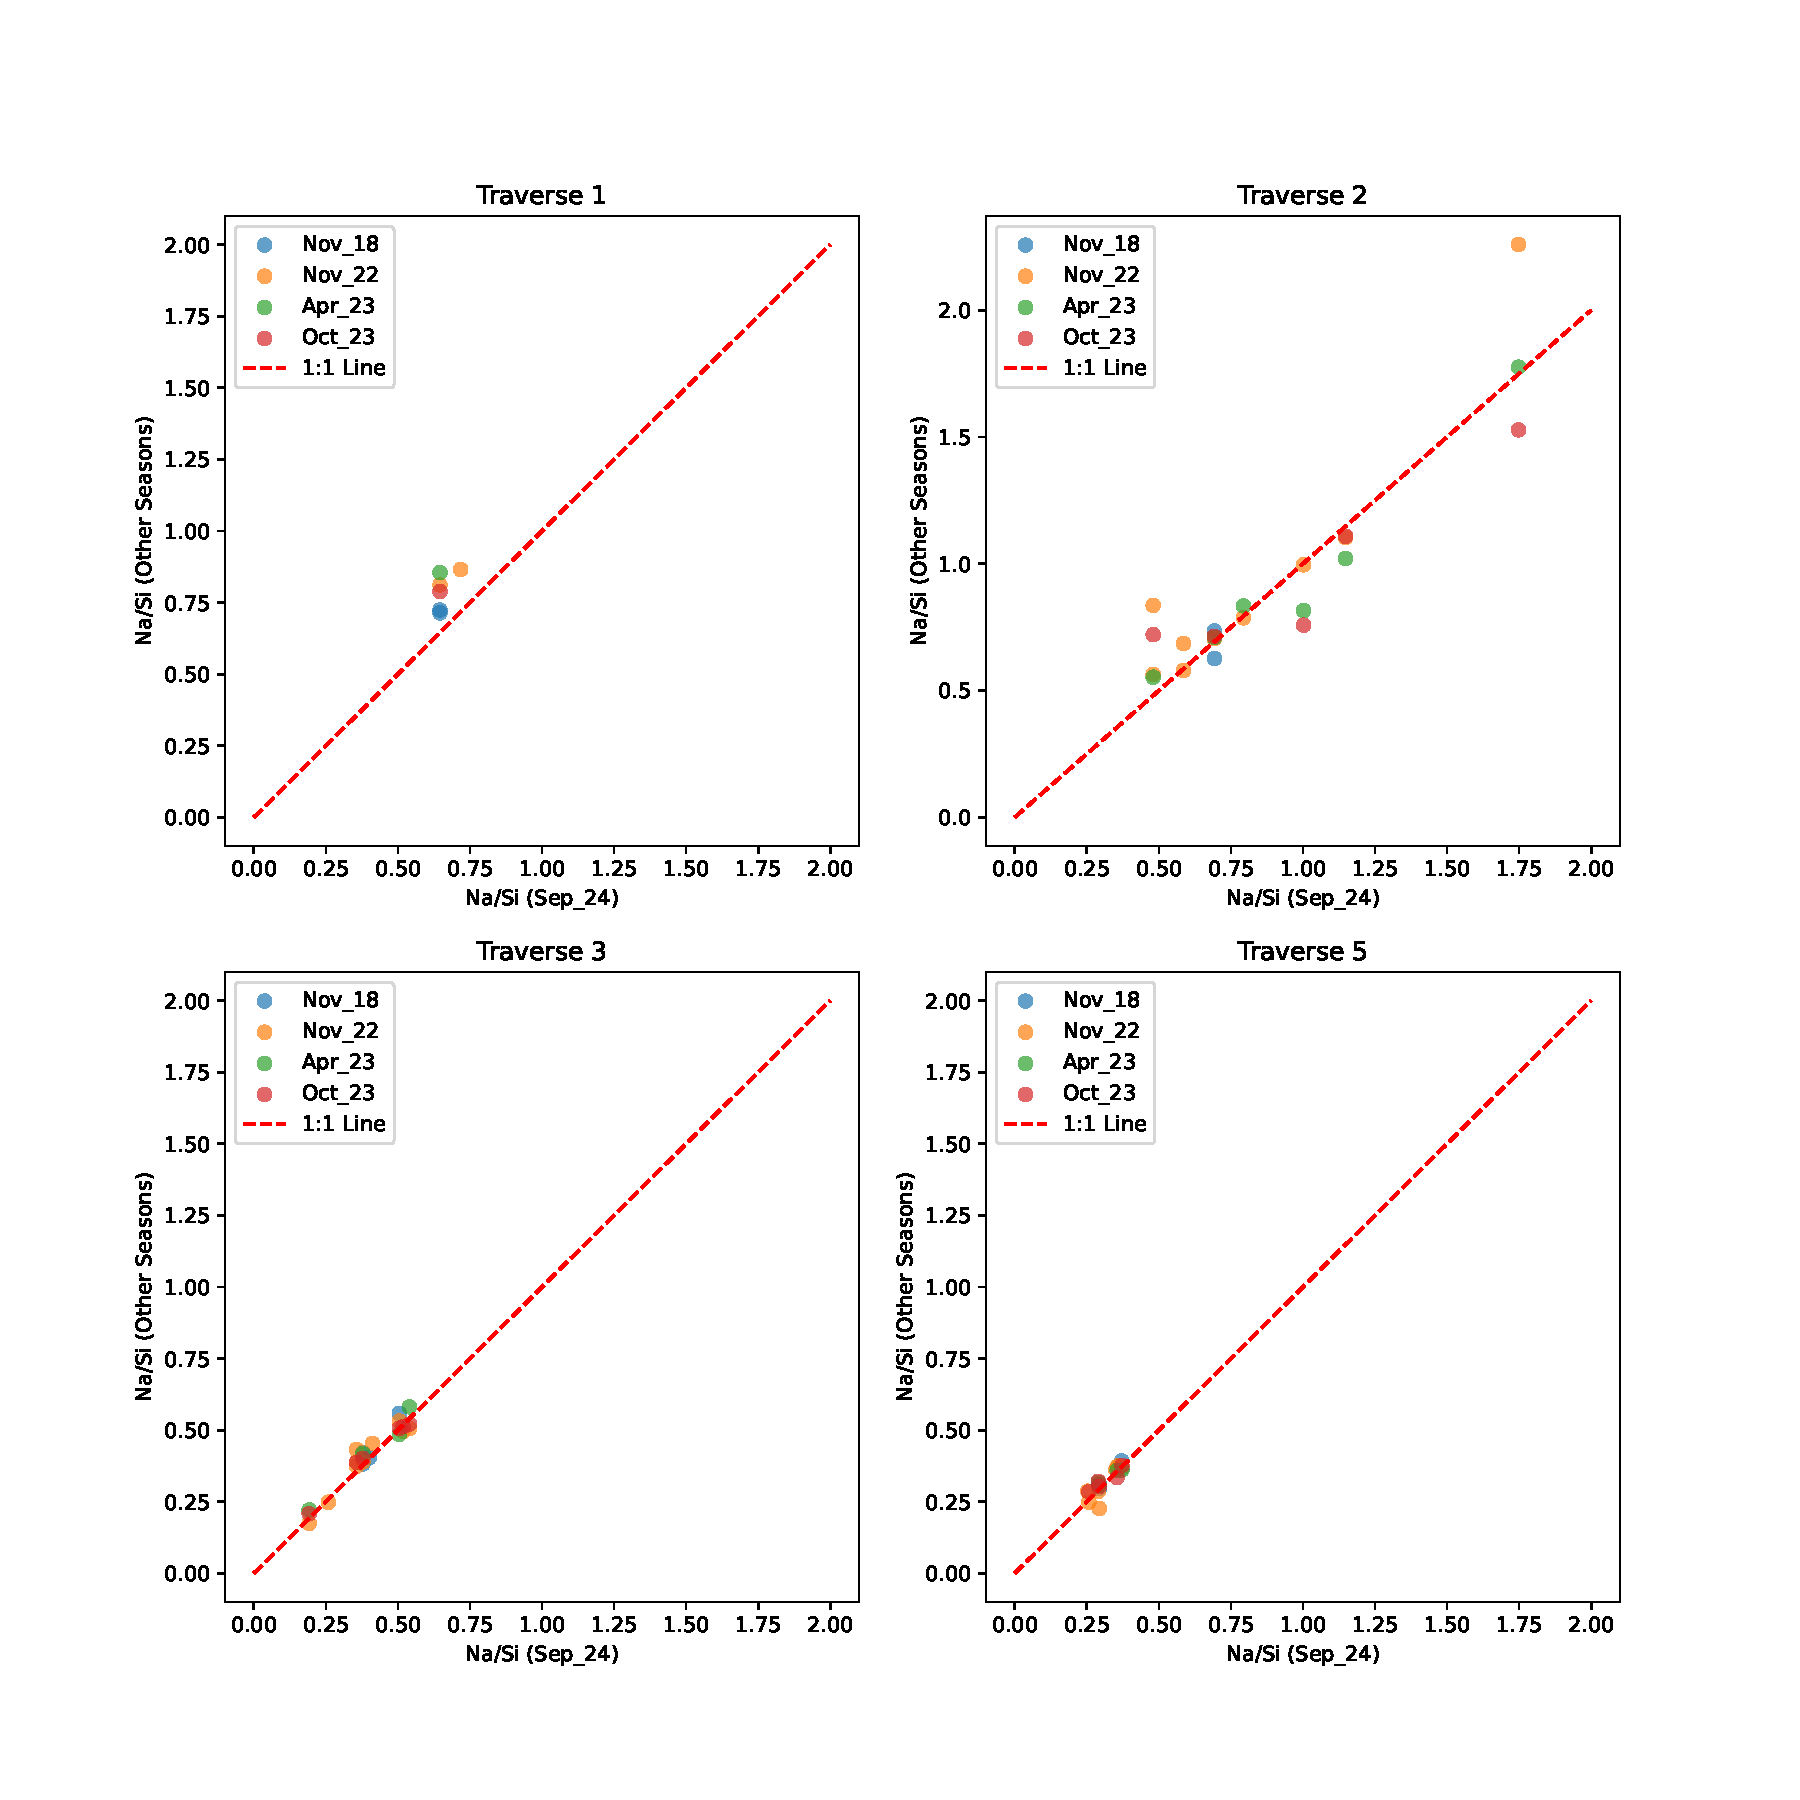
\includegraphics[width=\textwidth]{Na_Si_Seasons.pdf}
%     \caption{How Na/Si varies for different traverses. Traverse 4 is not plotted due to the lack of samples.}
%     \label{fig:spatial_changes_spring8}
% \end{figure}
% \FloatBarrier

% The scatter in these plots reflect temporal variability in the spring chemistry. Traverses 1 and 5 both display tight scatter, consistent with the notion that the flow paths here are consistently sampled. More notable here are the differences in Na/Si values between traverses. These how the spatial variability between traverses is more significant than the temporal variability. It is possible, and quite likely that all traverses flow paths are connected one to the other. When investigating model differences, however, a knowledge of which traverse accounts for what discrepancy allows for the contribution of spatial variation toward the overall interpretation to be taken into account.


% \subsection{Lithological Control on Spring Chemistry}

% Radiogenic strontium isotope analyses of springs show significant variation between different traverses. Sr isotope values of rain are consistent with the expected values for rainwater, with the exception of those sampled at low elevation (Galy, France-Lenord, Derry, 1999). The lowest Sr isotope value for rain is very close to the reported value for seawater, which is 0.70917 (Paytan et al, 2021). The rain samples with low strontium isotopic composition therefore indicate little contamination from dust or particles. Strontium isotope ratios used alongside strontium concentrations can be used to determine mixing between different endmembers (Faure, 1986; See Appendix). Plots of $\ddfrac{^{87}Sr}{^{86}Sr}$ against $\ddfrac{1}{Sr}$ that yield straight lines are indicative of mixing trends.


% \begin{figure}[p]
%     \centering
%     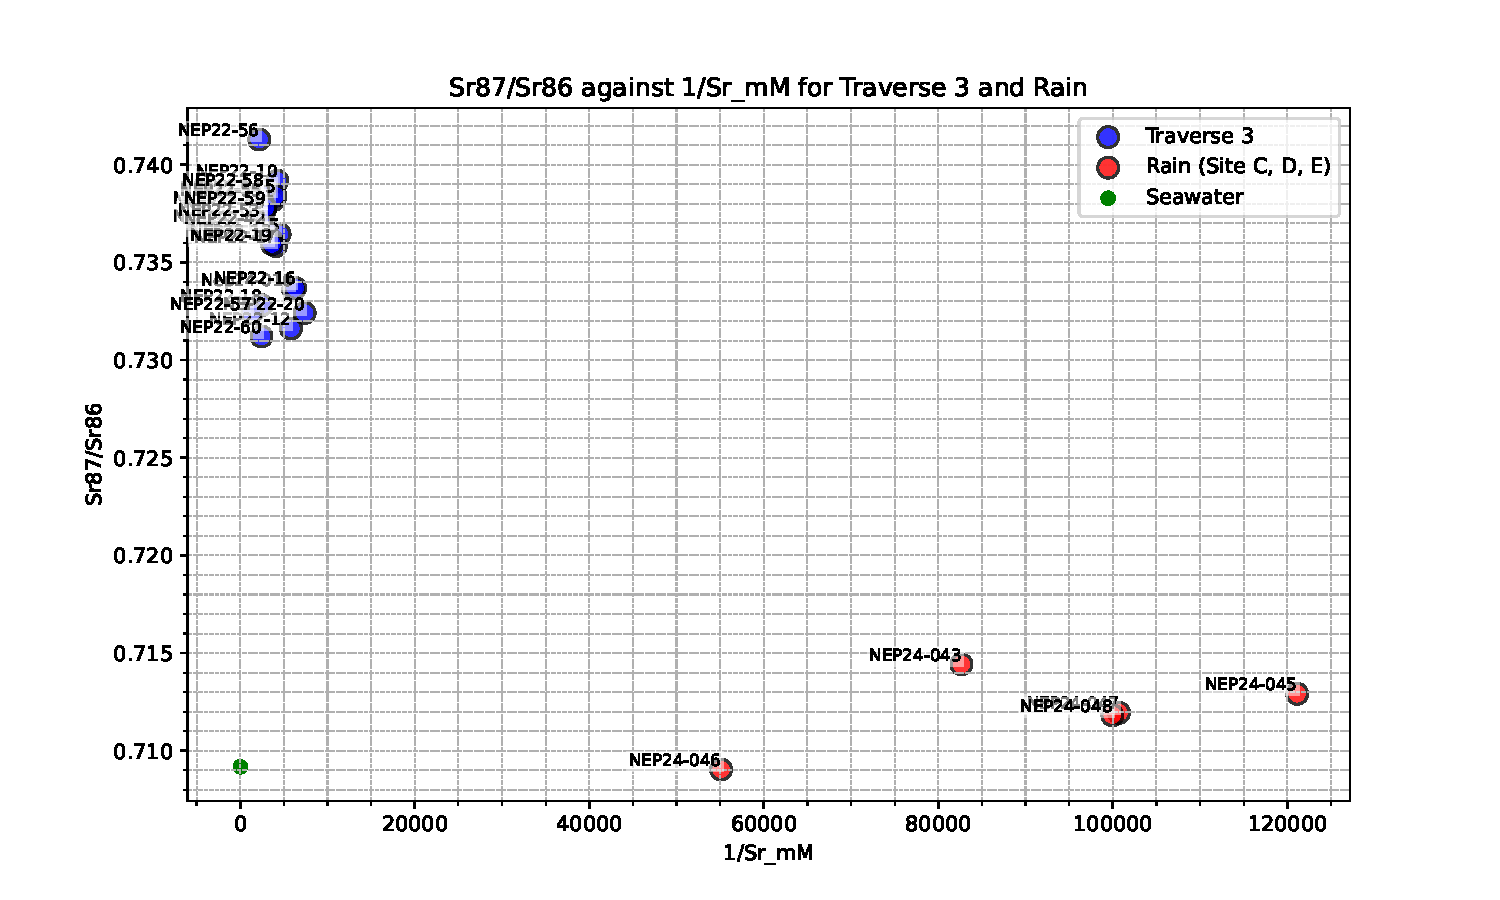
\includegraphics[width=\textwidth]{Sr87_Sr86_1Sr_Rain.pdf}
%     \caption{Strontium isotope differences display difference in lithology tapped in. Cite Quade and Tipper papers; Rain analysed for Sr isotopes and Cl. Something about contamination lower down; How samples of Traverse 3 compare to the rain samples}
%     \label{fig:discussion3}
% \end{figure}

% \FloatBarrier


% Comparing springs to rain in \ref{fig:discussion3}, the major control on spring chemistry does not appear to be the rain. Spring water mixing trends in $\ddfrac{^{87}Sr}{^{86}Sr}$ against $\ddfrac{1}{Sr}$ space are tightly scattered away from the rain. This suggests that rain input does not exert a significant control on the spring chemistry, which implies even the highest springs with the shortest flowpaths undergo significant weathering reactions with the rock. Instead, the water chemistry reflects that different traversal flowpaths sample lithologies that have different strontium isotopic composition. These variations are however within the range of Higher Himalayan Crystalline Series (HHCS) rocks found in the region, so this variation is to be expected (Tipper et al., 2006). It is unlikely that the source of the Sr isotopes is from the Lesser Himalayan Series (LHS) rocks, and the Main Central Thrust (MCT) is several km south of Melamchi.


